% $Header: /Users/joseph/Documents/LaTeX/beamer/solutions/conference-talks/conference-ornate-20min.en.tex,v 90e850259b8b 2007/01/28 20:48:30 tantau $

\documentclass[xcolor={usenames,dvipsnames}]{beamer}

% This file is a solution template for:

% - Talk at a conference/colloquium.
% - Talk length is about 20min.
% - Style is ornate.



% Copyright 2004 by Till Tantau <tantau@users.sourceforge.net>.
%
% In principle, this file can be redistributed and/or modified under
% the terms of the GNU Public License, version 2.
%
% However, this file is supposed to be a template to be modified
% for your own needs. For this reason, if you use this file as a
% template and not specifically distribute it as part of a another
% package/program, I grant the extra permission to freely copy and
% modify this file as you see fit and even to delete this copyright
% notice. 


\mode<presentation>
{
  \usetheme{CambridgeUS}
  % or ...

  \setbeamercovered{transparent}
  % or whatever (possibly just delete it)
  
\makeatletter
\setbeamertemplate{headline}{%
\leavevmode%
  \hbox{%
    \begin{beamercolorbox}[wd=.5\paperwidth,ht=2.25ex,dp=1ex]{section in head/foot}%
    \usebeamerfont{section in head/foot}\,\insertsection
    \end{beamercolorbox}%
    \begin{beamercolorbox}[wd=.5\paperwidth,ht=2.25ex,dp=1ex,right]{subsection in head/foot}%
    \usebeamerfont{section in head/foot}The ALICE Collaboration\,
    \end{beamercolorbox}%
  }
}
\makeatother
}

\usepackage[percent]{overpic}

\usepackage[english]{babel}
% or whatever

\usepackage[latin1]{inputenc}
% or whatever

\usepackage{times}
\usepackage[T1]{fontenc}
% Or whatever. Note that the encoding and the font should match. If T1
% does not look nice, try deleting the line with the fontenc.
%particles
\newcommand{\jpsi}{\rm J/$\psi$}
\newcommand{\psip}{$\psi^\prime$}
\newcommand{\jpsiDY}{\rm J/$\psi$\,/\,DY}
\newcommand{\chic}{$\chi_{\rm c}$}
\newcommand{\pip}{$\pi^{+}$}
\newcommand{\pim}{$\pi^{-}$}
\newcommand{\pizero}{$\pi^{0}$}
\newcommand{\kap}{K$^{+}$}
\newcommand{\kam}{K$^{-}$}
\newcommand{\pbar}{$\rm\overline{p}$}
\newcommand{\ccbar}{\ensuremath{\mathrm{c\overline{c}}}}
\newcommand{\bbbar}{\ensuremath{\mathrm{b\overline{b}}}}
\newcommand{\Dzero}{\ensuremath{\mathrm{D^{0}}}}
\newcommand{\Dzerobar}{\ensuremath{\mathrm{\overline{D}^{0}}}}
\newcommand{\Dpm}{\ensuremath{\mathrm{D^{\pm}}}}
\newcommand{\Ds}{\ensuremath{\mathrm{D_{s}^{\pm}}}}
\newcommand{\Dstar}{\ensuremath{\mathrm{D^{*\pm}}}}

%collision systems
\newcommand{\pp}{pp}
\newcommand{\pPb}{p--Pb}
\newcommand{\PbPb}{Pb--Pb}

%detectors
\newcommand{\ezdc}{$E_{\rm ZDC}$}

%units
\newcommand{\GeVc}{GeV/$c$}
\newcommand{\GeVcsq}{GeV/$c^2$}

%others
\newcommand{\degree}{$^{\rm o}$}
\newcommand{\s}{\ensuremath{\sqrt{s}}}
\newcommand{\snn}{\ensuremath{\sqrt{s_{\rm NN}}}}
\newcommand{\y}{\ensuremath{y}}
\newcommand{\pt}{\ensuremath{p_{\rm T}}}
\newcommand{\dedx}{d$E$/d$x$}
\newcommand{\dndy}{d$N$/d$y$}
\newcommand{\dndydpt}{${\rm d}^2N/({\rm d}y {\rm d}p_{\rm t})$}
\newcommand{\zpar}{\ensuremath{z_{||}}}
\newcommand{\zpargen}{\ensuremath{z_{||}^{\mathrm{part}}}}
\newcommand{\zpardet}{\ensuremath{z_{||}^{\mathrm{det}}}}
\newcommand{\ptchjet}{\ensuremath{p_{\mathrm{T,ch\, jet}}}}
\newcommand{\ptjet}{\ensuremath{p_{\mathrm{T,jet}}}}
\newcommand{\ptchjetgen}{\ensuremath{p_{\mathrm{T,ch\,jet}}^{\mathrm{part}}}}
\newcommand{\ptchjetdet}{\ensuremath{p_{\mathrm{T,ch\,jet}}^{\mathrm{det}}}}
\newcommand{\ptd}{\ensuremath{p_{\mathrm{T,D}}}}
\newcommand{\ptdgen}{\ensuremath{p_{\mathrm{T,D}}^{\mathrm{part}}}}
\newcommand{\ptddet}{\ensuremath{p_{\mathrm{T,D}}^{\mathrm{det}}}}
\newcommand{\antikt}{anti-\ensuremath{k_{\mathrm{T}}}}
\newcommand{\Antikt}{Anti-\ensuremath{k_{\mathrm{T}}}}
\newcommand{\kt}{\ensuremath{k_{\mathrm{T}}}}
\newcommand{\pthard}{\ensuremath{p_{\mathrm{T,hard}}}}

\title[D-tagged jets in pp collisions at 7 TeV] % (optional, use only with long paper titles)
{D-meson tagged jets in pp collisions at 7 TeV}

\author[Salvatore Aiola]% (optional, use only with lots of authors)
{Salvatore Aiola (Yale University),\\
on behalf of the ALICE Collaboration\\
\bigskip

\includegraphics[height=2cm]{img/yale}\quad

\includegraphics[height=2cm]{img/alice}}
% - Give the names in the same order as the appear in the paper.
% - Use the \inst{?} command only if the authors have different
%   affiliation.

\institute[Yale University] % (optional, but mostly needed)


\date[Hot Quarks 2016] % (optional, should be abbreviation of conference name)
{Hot Quarks 2016, September 12-17, South Padre Island, TX}
% - Either use conference name or its abbreviation.
% - Not really informative to the audience, more for people (including
%   yourself) who are reading the slides online

\subject{High-Energy Physics}
% This is only inserted into the PDF information catalog. Can be left
% out. 



% If you have a file called "university-logo-filename.xxx", where xxx
% is a graphic format that can be processed by latex or pdflatex,
% resp., then you can add a logo as follows:

% \pgfdeclareimage[height=0.5cm]{university-logo}{university-logo-filename}
% \logo{\pgfuseimage{university-logo}}


% If you wish to uncover everything in a step-wise fashion, uncomment
% the following command: 

%\beamerdefaultoverlayspecification{<+->}


\begin{document}

\begin{frame}
  \titlepage
\end{frame}

\begin{frame}{Outline}
  \tableofcontents
  % You might wish to add the option [pausesections]
\end{frame}


% Structuring a talk is a difficult task and the following structure
% may not be suitable. Here are some rules that apply for this
% solution: 

% - Exactly two or three sections (other than the summary).
% - At *most* three subsections per section.
% - Talk about 30s to 2min per frame. So there should be between about
%   15 and 30 frames, all told.

% - A conference audience is likely to know very little of what you
%   are going to talk about. So *simplify*!
% - In a 20min talk, getting the main ideas across is hard
%   enough. Leave out details, even if it means being less precise than
%   you think necessary.
% - If you omit details that are vital to the proof/implementation,
%   just say so once. Everybody will be happy with that.

\section{Physics Motivations}

\subsection{Charm and pQCD}
\begin{frame}{D-Meson Cross Sections}
\begin{columns}
\column{.5\textwidth}
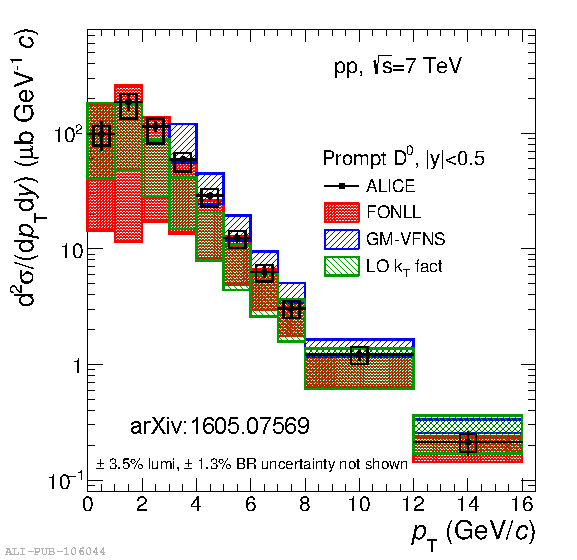
\includegraphics[width=\textwidth]{img/ALICE_D0Meson}

\column{.5\textwidth}
\textbf{\alert{Sensitive test of pQCD}}
\begin{itemize}
\item D mesons measured down to \alert{$\ptd=0$~\GeVc}
\item \alert{$Q^2\approx m_{\rm c}^2 \neq 0$}
\begin{itemize}
\item[$\rightarrow$] pQCD is still applicable even for $\ptd\approx0$~\GeVc
\end{itemize}
\item large theoretical uncertainties at low \ptd $\rightarrow$ \alert{small $Q^2$, $x$}
\begin{itemize}
\item renormalization scale
\item gluon PDFs
\end{itemize}
\end{itemize}
\end{columns}
\medskip
\alert{\textbf{D-Tagged Jets}: kinematics closer to the originating parton} $\rightarrow$ reduced dependence on the fragmentation function
\end{frame}

\begin{frame}{D-Tagged Jets}
\begin{columns}
\column{.5\textwidth}
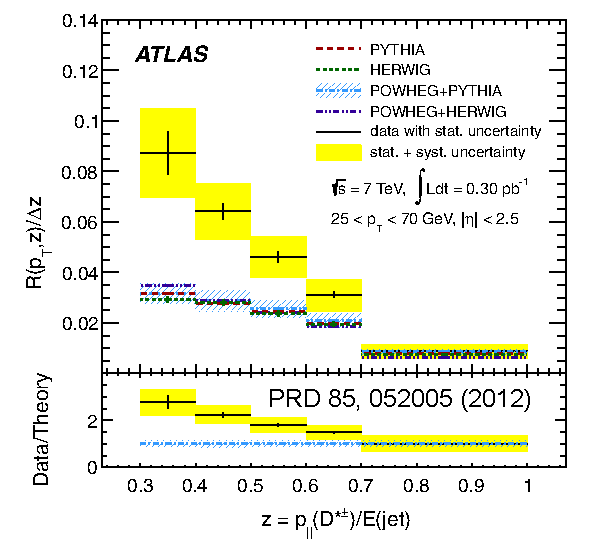
\includegraphics[width=\textwidth]{img/ATLAS_DStarJets}
\column{.5\textwidth}
\begin{itemize}
\item \alert{Few measurements} of D-tagged jets in recent years
\begin{itemize}
\setlength\itemsep{0em}
\item {\scriptsize \textbf{STAR}: PRD 79 (2009) 112006}
\item {\scriptsize \textbf{ATLAS}: PRD 85 (2012) 052005}
\end{itemize}
\item \alert{Large discrepancy} with pQCD-based MC generators
\item D-tagged jets can help to pin-point weaknesses in our understanding of QCD
\begin{itemize}
\item production mechanism?
\item fragmentation functions?
\end{itemize}
\end{itemize}
\end{columns}

\smallskip
{\small ALICE expected kinematical reach:}
\begin{itemize}
{\small \item $\s=7$~TeV $\rightarrow$ \emph{charged jets} with \alert{$5<\ptchjet<24$~\GeVc} (this analysis)}
{\small \item $\s=8$,~$13$~TeV $\rightarrow$ \emph{full jets} with \alert{smaller $z$ for $\ptjet \gtrsim 20$~\GeVc}}
\end{itemize}
\end{frame}

\subsection{Charm and the QGP}
\begin{frame}{Probe of the Quark-Gluon Plasma}
\begin{columns}
\column{.56\textwidth}
\textbf{\alert{Self-produced probe}}
\begin{itemize}
\item c quarks are \alert{produced early} in the collision
\item Energy loss in the medium
\begin{columns}[T]
\column{.4\textwidth}
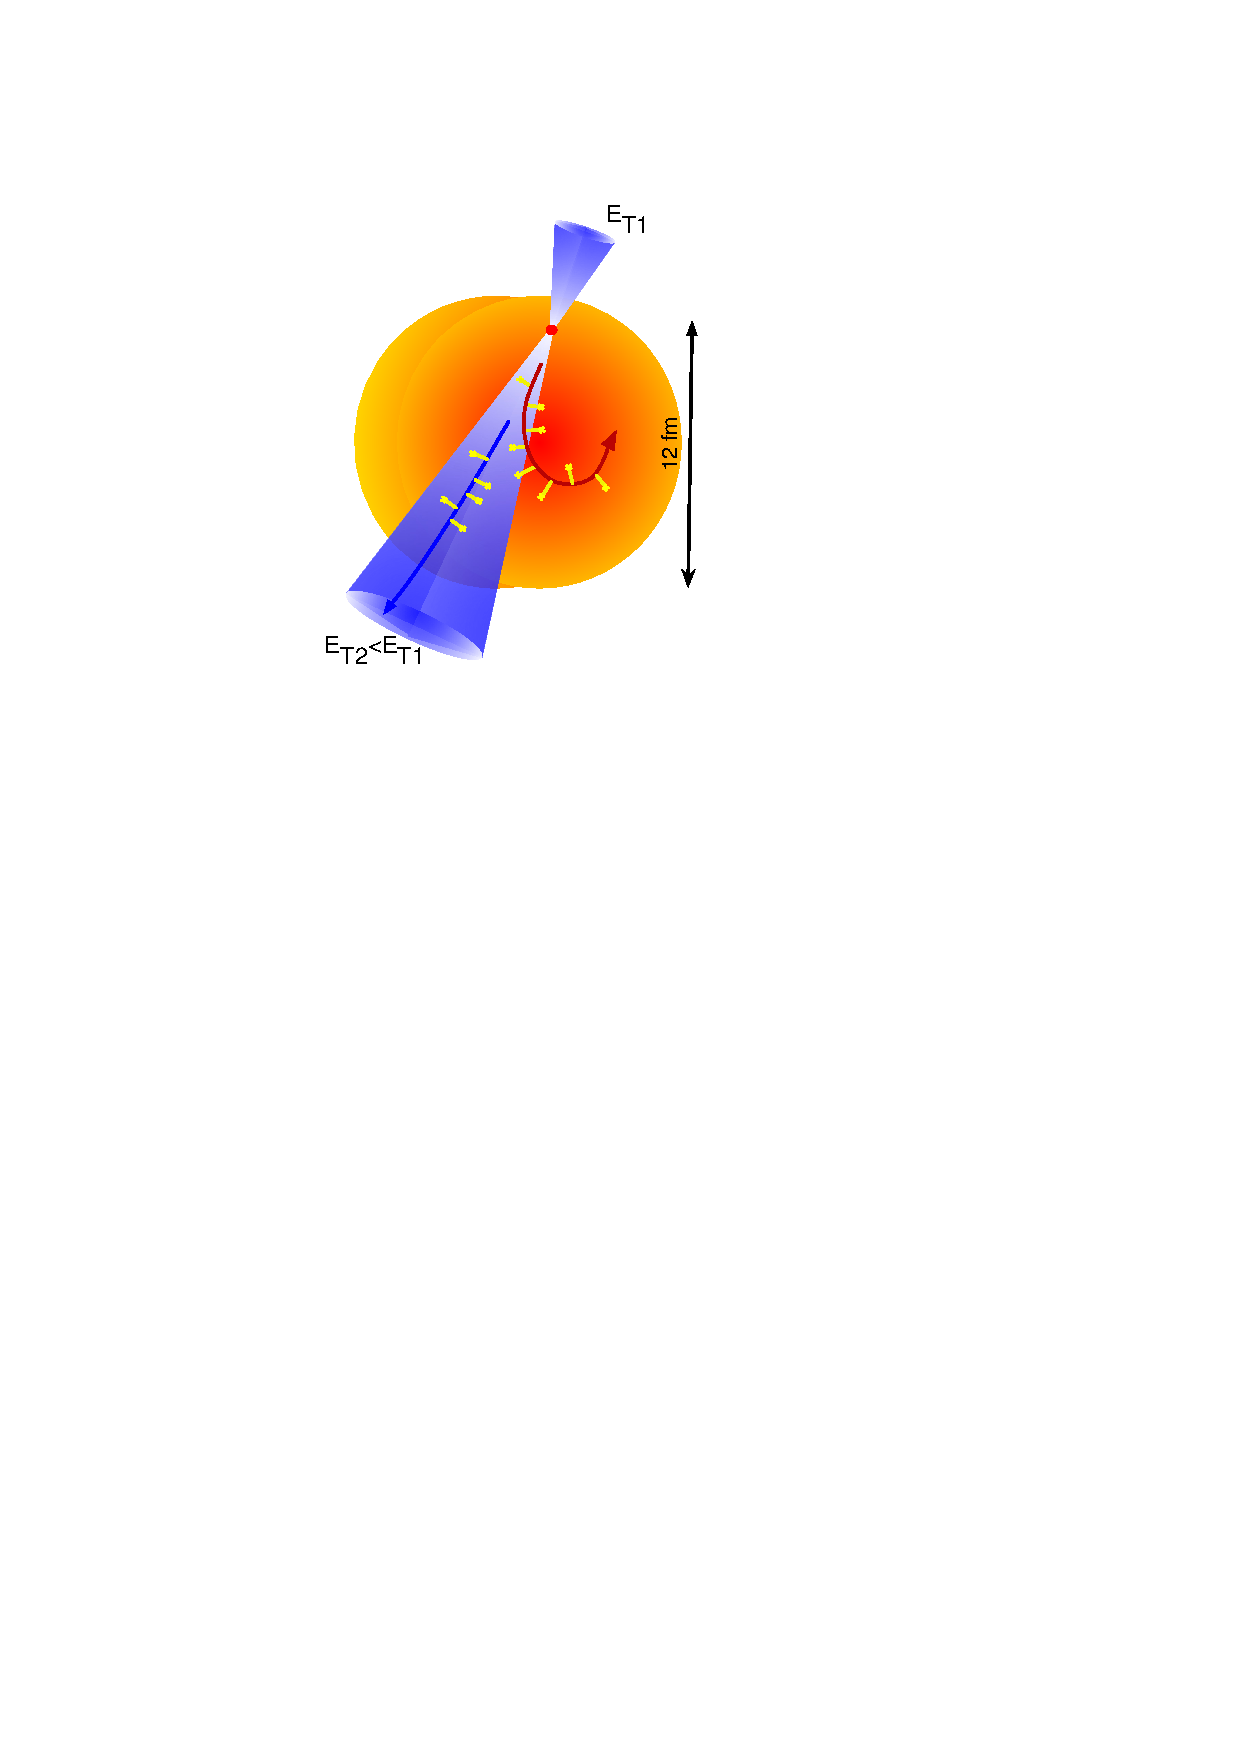
\includegraphics[width=\textwidth]{img/jetquenching}
\column{.6\textwidth}
\begin{itemize}
\setlength\itemsep{0em}
\item elastic collisions
\item radiative \\
$\rightarrow$ \alert{dead-cone effect}\footnote[frame,1]{Dokshitzer and Kharzeev, PLB 519 (2001) 199} \\
$m_{\rm c} > 0$ suppresses small angle radiation
\end{itemize}
\end{columns}
\end{itemize}

\column{.44\textwidth}
\begin{overpic}[width=\textwidth, trim=1 0 13 0, clip]{img/ALICE_DMesonRAA}
 \put (25,40) {{\footnotesize JHEP1603 (2016) 081}}
\end{overpic}
\end{columns}
\begin{itemize}
\item Hint of slightly \alert{smaller suppression} compared to pions at low \pt
\end{itemize}
\smallskip
\alert{\textbf{D-Tagged Jets}: kinematics closer to the originating parton} $\rightarrow$ can magnify dead cone effect at low \ptjet
\end{frame}

\section{Analysis Overview}

\subsection{ALICE at the LHC}
\begin{frame}{ALICE at the LHC}
\begin{columns}

\column{.58\textwidth}
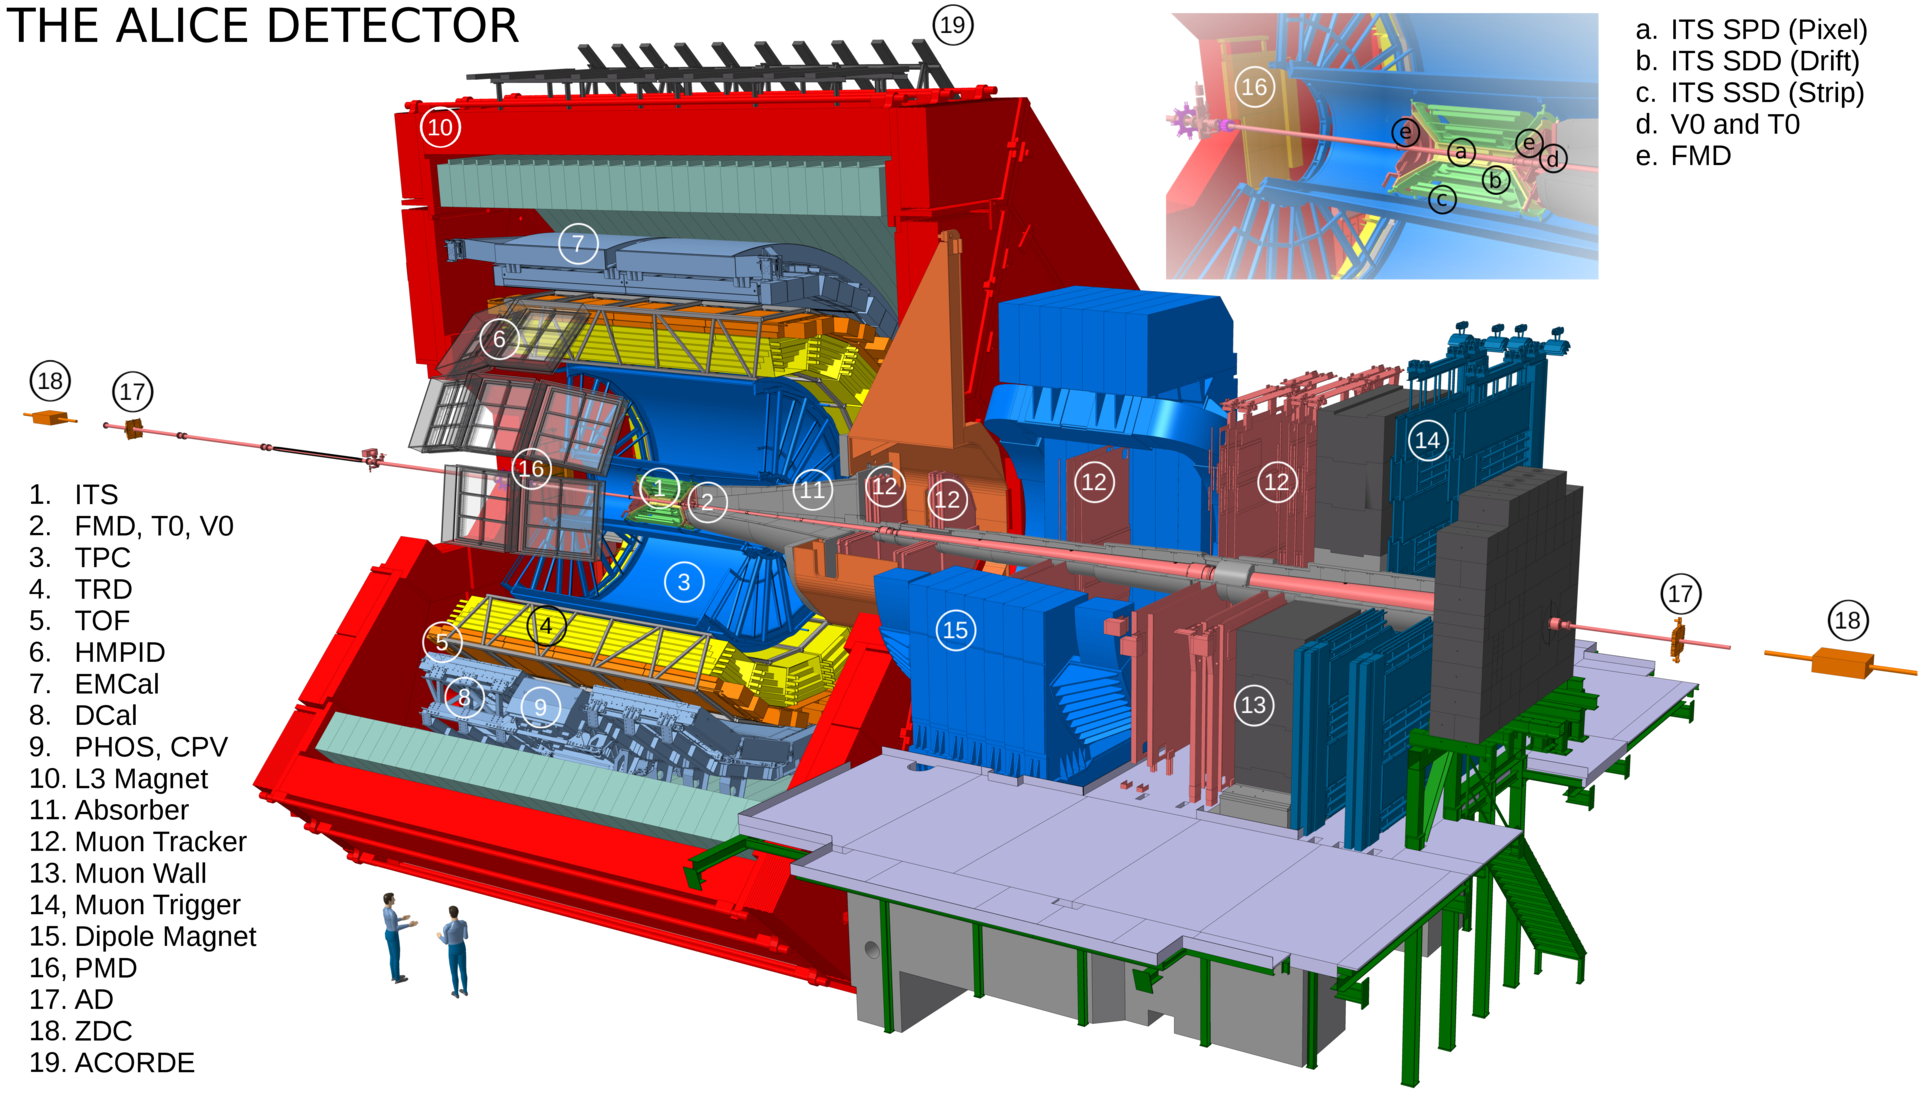
\includegraphics[width=\textwidth]{img/ALICE_Schematics}

\column{.42\textwidth}
\begin{itemize}
\item Important features
\begin{itemize}
\item \alert{PID} \\
(e, $\mu$, $\pi$, K, p, d, ${}^3$He)
\item \alert{low-momentum tracking} ($\pt > 0.15$~\GeVc)
\end{itemize}
\item \alert{D mesons} via hadronic decays (ITS, TPC, TOF)
\begin{itemize}
\item PID, topological cuts
\item invariant mass analysis
\end{itemize}
\end{itemize}
\end{columns}
\begin{itemize}
\item \alert{Jet reconstruction} using \antikt\ algorithm
\begin{itemize}
\item \textcolor{ForestGreen}{charged constituents} (ITS, TPC) $\rightarrow$ \emph{charged jets} (this analysis)
\item add \textcolor{NavyBlue}{neutral constituents} (EMCal, DCal) $\rightarrow$ \emph{full jets} 
\end{itemize}
\end{itemize}
\end{frame}

\subsection{D-meson jet tagging}
\begin{frame}{D-meson jet tagging}

\begin{columns}

\column{0.6\textwidth}
\begin{enumerate}
\item For each \Dzero\ meson candidate that passes \alert{PID} and \alert{topological} cuts utilize \antikt\ \alert{jet finding}\\ (\pt\ recombination scheme)
\begin{itemize}
\item \Dzero\ candidate 4-momentum
\item all other reconstructed tracks
\item exclude candidate daughters
\end{itemize}
\item Combinatorial background from random $\mathrm{K}\pi$ pairs 
\begin{itemize}
\item[$\rightarrow$] \alert{invariant mass analysis} to extract signal
\end{itemize}
\end{enumerate}

\column{0.4\textwidth}
\begin{overpic}[width=\textwidth, trim=190 0 190 0, clip]{img/ALICE_D0InvMass}
 \put (25,35) {{\scriptsize JHEP 1201 (2012) 128}}
\end{overpic}
\end{columns}
\bigskip
\textbf{\alert{\Dzero(\Dzerobar) meson}}
\begin{itemize}
\item $M=1.865$~\GeVcsq, $c\tau=123\,\mu\mathrm{m}$ 
\item Decay: \Dzero$\rightarrow\mathrm{K}^+\pi^-$ and c.c. with ${\rm BR}=3.88\%$
\end{itemize}
\end{frame}


\section{Detector Perfomance}

\subsection{D-Tagged Jet Reconstruction Efficiency}
\begin{frame}{D-Tagged Jet Reconstruction Efficiency}
\alert{PYTHIA6} Perugia-2011 + \alert{GEANT3} with detailed description of ALICE
\begin{columns}
\column{.60\textwidth}
\begin{overpic}[width=\textwidth, trim=0 0 38 0, clip]{img/HQ16_Simulation_EfficiencyVsDPt}
\end{overpic}
\column{.40\textwidth}
\begin{itemize}
\item Dominated by \\ \textcolor{NavyBlue}{\Dzero\ reconstruction efficiency}
\item \alert{Strong increase with \ptd\ at low \ptd} \\
$\rightarrow$ topological cuts on the secondary vertex, tighter at low \ptd\
\end{itemize}
\end{columns}
\bigskip
\textcolor{ForestGreen}{No dependence on the \ptchjet}: simplifies corrections and reduces systematic uncertainties 
\end{frame}

\subsection[JES shift and \pt\ resolution]{Jet Energy Scale shift and \pt\ resolution}

\begin{frame}[t]{Jet Energy Scale shift and \pt\ resolution}
\begin{columns}
\column{.47\textwidth}
\begin{overpic}[width=\textwidth]{img/ALICE_JetRes}
\put (-3,4) {{\tiny PRD 91 (2015) 112012}}
\end{overpic}\\
\medskip
{\small
\textcolor{BrickRed}{
\textbf{Inclusive Charged Jets} \\
\medskip
$\mu [(\ptchjetdet-\ptchjetgen)/\ptchjetgen]\approx -3\%$ \\
\smallskip
$\sigma[(\ptchjetdet-\ptchjetgen)/\ptchjetgen]\approx17\%$
}}
\column{.53\textwidth}
\medskip
\begin{overpic}[width=\textwidth, trim=0 9 30 22, clip]{img/HQ16_Simulation_DetectorResponse}
\end{overpic}\\
\raggedleft
{\small
\textcolor{NavyBlue}{
\textbf{D-Tagged Charged Jets}\\
\medskip
$\mu[(\ptchjetdet-\ptchjetgen)/\ptchjetgen]\approx -3\%$ \\
\smallskip
$\sigma[(\ptchjetdet-\ptchjetgen)/\ptchjetgen]\approx11\%$
}}
\end{columns}
\bigskip
\centering
\textbf{slightly better \ptchjet\ resolution due to the D-meson requirement}
\end{frame}

\begin{frame}{JES shift and \pt\ resolution: \pt-dependence}
\begin{columns}
\column{.50\textwidth}
\centering
\textbf{JES shift}\\
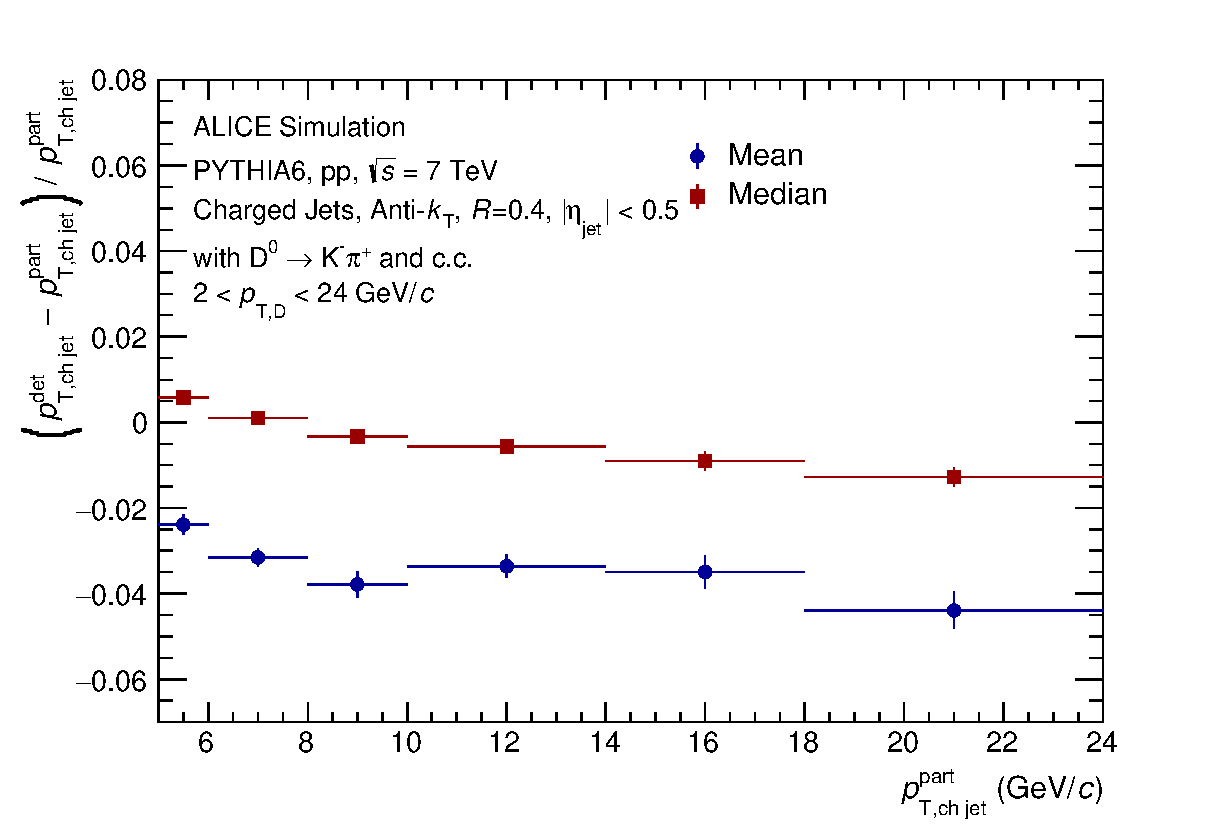
\includegraphics[width=\textwidth]{img/HQ16_Simulation_EnergyScaleShift}
\column{.50\textwidth}
\centering
\textbf{\ptchjet\ resolution} \\
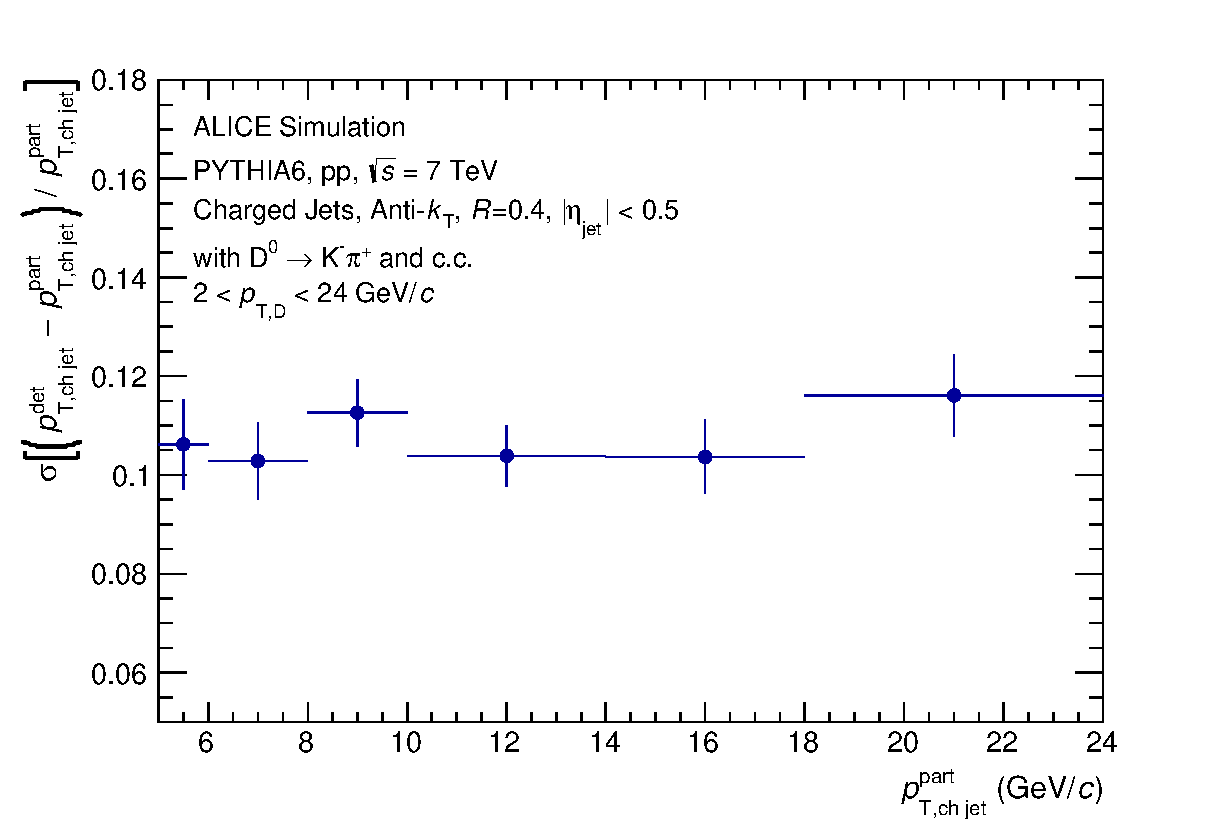
\includegraphics[width=\textwidth]{img/HQ16_Simulation_Resolution}
\end{columns}
\medskip
\begin{itemize}
\item JES shift and \ptchjet\ resolution dominated by \alert{tracking efficiency}
\item \alert{No significant \pt-dependence} in the range $5<\ptchjet<24$ \GeVc
\end{itemize}
\end{frame}

\section{Signal Extraction}

\subsection{D-tagged jet signal extraction}

\begin{frame}[t]{Signal extraction}
\begin{columns}[T]
\column{.5\textwidth}
\begin{overpic}[width=\textwidth, trim=0 0 0 50, clip]{img/HQ16_Simulation_InvMassSB}
\end{overpic}
\column{.5\textwidth}
\textbf{\alert{Three methods}}
\begin{enumerate}
\item \textcolor{BrickRed}{Side-Band (S-B) background subtraction}
\item \textcolor{ForestGreen}{Like-Sign (L-S) background subtraction}
\item \textcolor{NavyBlue}{Invariant Mass Fit in bins of \ptchjet}
\end{enumerate}
\end{columns}
\end{frame}

\begin{frame}[t]{Signal extraction: S-B method}
\begin{columns}[T]
\column{.50\textwidth}
\begin{overpic}[width=\textwidth, trim=0 0 0 50, clip]{img/HQ16_Simulation_InvMassSB}
\end{overpic}
\column{.50\textwidth}
\textbf{\textcolor{BrickRed}{Method 1: Side-Band (S-B)}}
\begin{enumerate}
\item Fill D-meson invariant mass distributions in bins of \alert{\ptd}
\item $N(\ptchjet, \ptd)$ distributions in
\medskip
\textcolor{NavyBlue}{\textbf{Peak Area}
{\scriptsize $|M_{\rm K\pi} - M_{\rm fit}| <2\sigma$}\\ 
\smallskip
$N_{\rm sig+bkg} (\ptchjet, \ptd)$}
\medskip
\textcolor{BrickRed}{\textbf{Side Bands}
{\scriptsize $8\sigma <|M_{\rm K\pi} - M_{\rm fit}| < 4\sigma$}\\ 
\smallskip
$N_{\rm bkg, SB} (\ptchjet, \ptd)$}
\end{enumerate}
\end{columns}
\begin{enumerate}
\setcounter{enumi}{2}
\item Apply \textcolor{VioletRed}{efficiency correction} and \textcolor{YellowOrange}{integrate in \ptd}
{\small $$N_{\rm signal} (\ptchjet)=\textcolor{YellowOrange}{\sum_{\ptd}} \textcolor{VioletRed}{\frac{1}{\epsilon(\ptd)}} [\textcolor{NavyBlue}{N_{\rm sig+bkg}(\ptchjet, \ptd)} - \textcolor{BrickRed}{N_{\rm bkg,SB}(\ptchjet, \ptd)}]$$}
\end{enumerate}
\end{frame}

\begin{frame}[t]{Signal extraction: L-S method}
\begin{columns}[T]
\column{.50\textwidth}
\begin{overpic}[width=\textwidth, trim=0 0 0 50, clip]{img/HQ16_Simulation_InvMassSB}
\end{overpic}
\column{.50\textwidth}
\textbf{\textcolor{ForestGreen}{Method 2: Like-Sign (L-S)}}
\begin{enumerate}
\item Fill D-meson invariant mass distributions in bins of \alert{\ptd}
\item $N(\ptchjet, \ptd)$ distributions in
\medskip
\textcolor{NavyBlue}{\textbf{U-S peak area} {\footnotesize $|M_{\rm K\pi} - M_{\rm fit}| <2\sigma$}\\ 
\smallskip
{\small $N_{\rm sig+bkg} (\ptchjet, \ptd)$}}
\medskip
\textcolor{ForestGreen}{\textbf{L-S peak area} {\footnotesize $|M_{\rm K\pi} - M_{\rm fit}| <2\sigma$}\\ 
\smallskip
{\small $N_{\rm bkg, LS} (\ptchjet, \ptd)$}}
\end{enumerate}
\end{columns}
\begin{enumerate}
\setcounter{enumi}{2}
\item Apply \textcolor{VioletRed}{efficiency correction} and \textcolor{YellowOrange}{integrate in \ptd}
{\small $$N_{\rm signal} (\ptchjet)=\textcolor{YellowOrange}{\sum_{\ptd}} \textcolor{VioletRed}{\frac{1}{\epsilon(\ptd)}} [\textcolor{NavyBlue}{N_{\rm sig+bkg}(\ptchjet, \ptd)} - \textcolor{ForestGreen}{N_{\rm bkg,LS}(\ptchjet, \ptd)}]$$}
\end{enumerate}
\end{frame}

\begin{frame}[t]{Signal extraction: invariant mass fit}
\begin{columns}[T]
\column{.5\textwidth}
\begin{overpic}[width=\textwidth, trim=0 0 0 50, clip]{img/HQ16_Simulation_InvMassSB}
\end{overpic}
\column{.5\textwidth}
\textbf{\textcolor{NavyBlue}{Method 3: invariant mass fit}}
\begin{enumerate}
\item Fill D-meson invariant mass distributions in bins of \alert{\ptchjet}
\item \textbf{Fit invariant mass distributions} with a \\ Gaussian (\textcolor{NavyBlue}{signal}) + exponential (\textcolor{BrickRed}{background})
\item Extract $N_{\rm signal} (\ptchjet)$ from fit parameters
\end{enumerate}
\end{columns}
\begin{itemize}
\item The correction for the D-tagged jet reconstruction efficiency must be applied as a weight when filling the invariant mass plots
\end{itemize}
\end{frame}

\subsection{Method comparison}
\begin{frame}{Method comparison}
\begin{columns}
\column{.55\textwidth}
\begin{overpic}[width=\textwidth, trim=0 0 50 0, clip]{img/HQ16_Simulation_MethodComparison}
\end{overpic}
\column{.45\textwidth}
\begin{itemize}
\item PYTHIA6 Perugia-2011 and GEANT3
\medskip
\item D-tagged jet signal yields extracted using the  \textbf{\textcolor{NavyBlue}{invariant mass fit}}, \textbf{\textcolor{BrickRed}{Side-Band}} 
and \textbf{\textcolor{ForestGreen}{Like-Sign}} methods are compared with the \textbf{\textcolor{gray}{MC truth}}
\medskip
\item All methods \textbf{agree well} with the MC truth within their statistical uncertainties
\end{itemize}
\end{columns}
\end{frame}

\subsection{Statistical precision}
\begin{frame}{Statistical precision}
\begin{columns}
\column{.55\textwidth}
\begin{overpic}[width=\textwidth, trim=0 0 50 30, clip]{img/HQ16_Simulation_UncertaintyComparison}
\end{overpic}
\column{.45\textwidth}
\begin{itemize}
\item The methods differ also in their \alert{statistical precision}
\item[$\rightarrow$] \textcolor{ForestGreen}{larger uncertainties for \textbf{L-S}}
\item The \alert{efficiency correction} alters the relative contribution of D-mesons with different \pt
\item[$\rightarrow$] the relative statistical uncertainty increases
\end{itemize}
\end{columns}

\end{frame}

\section*{Summary}

\subsection*{Conclusions}
\begin{frame}{Conclusions}
\begin{itemize}
\item The measurement of the charm cross-section and fragmentation function provide important tools for
\textbf{\alert{testing pQCD}} (\pp) and \textbf{\alert{probing the QGP}} (\PbPb)
\item 3 different techniques have been developed to extract the D-tagged jet yield:
\begin{itemize}
\item Bin counting in the peak area w/ \textbf{\textcolor{BrickRed}{Side-Band}} background subtraction
\item Bin counting in the peak area w/ \textbf{\textcolor{ForestGreen}{Like-Sign}} background subtraction
\item \textbf{\textcolor{NavyBlue}{Invariant mass fit}} in bins of \ptchjet
\end{itemize}
\item Proved to be \alert{feasible} and \alert{successfully tested} in Monte Carlo
\item The pros and cons of each technique is being assessed
\item \textbf{\alert{Now looking forward to finalize the analysis on real data!}}
\end{itemize}
\end{frame}

\subsection*{Stay Tuned: Work In Progress!}
\begin{frame}{Stay Tuned: Work In Progress!}
\begin{columns}
\column{.55\textwidth}
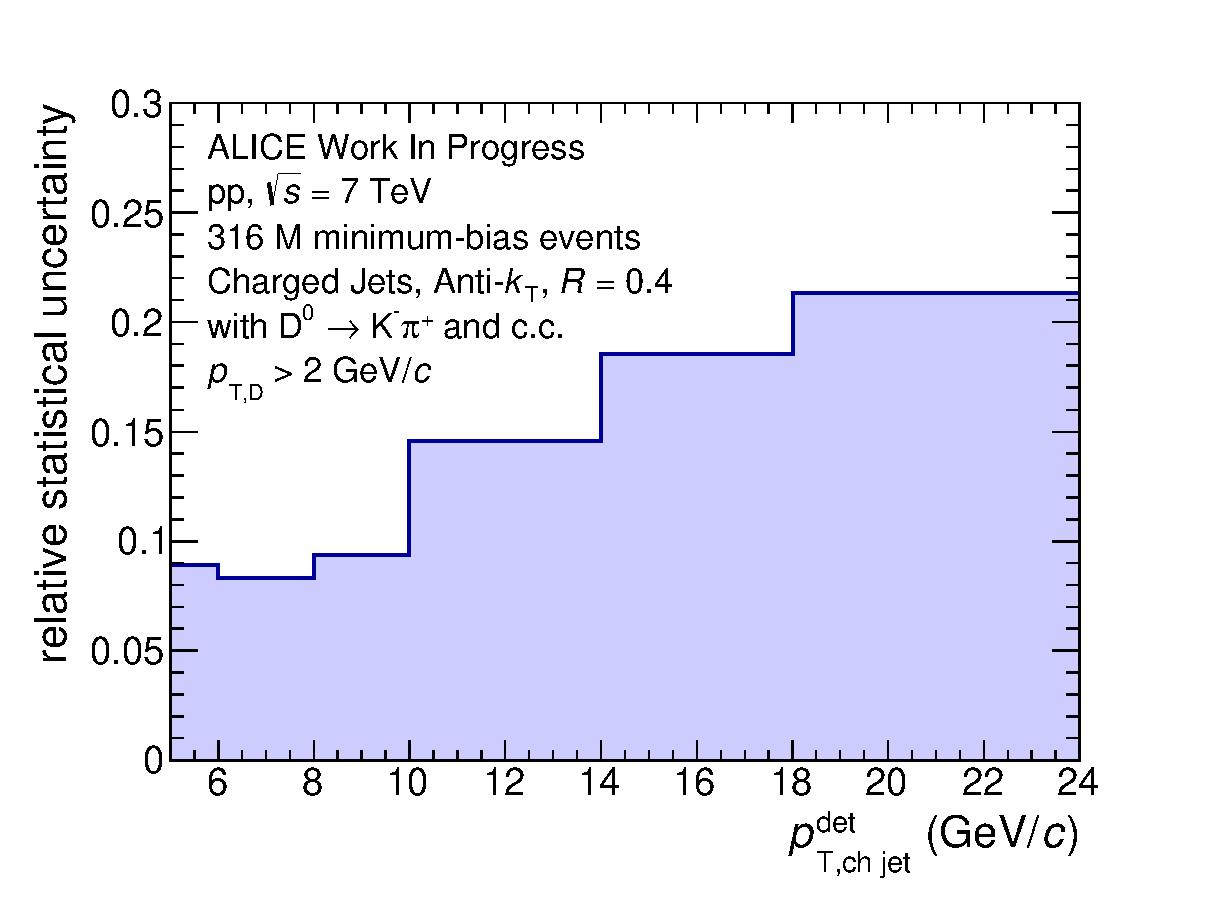
\includegraphics[width=\textwidth]{img/HQ16_WorkInProgress_StatisticalUncertainty} 

\column{.45\textwidth}
\begin{itemize}
\item The analysis is being performed using data collected by ALICE with pp collisions at $\s=7$~TeV
\item A preliminary look at the available statistics in 2010 data has given promising expectations
\item \textbf{\alert{Look out for new results being made public soon!}}
\end{itemize}
\end{columns}
\end{frame}

% All of the following is optional and typically not needed. 
%\appendix
%\section<presentation>*{\appendixname}
%\subsection<presentation>*{Backup}

%\begin{frame}
 % \frametitle<presentation>{Backup 1}    
%\end{frame}

\end{document}
